The web-based implementation of GrandeOmega features, at its core, a generic code interpreter which takes as input a specification of one or more programming languages, and yields the following as output:

\begin{itemize}[noitemsep]
	\item an interactive, assistive code-editor (Figure \ref{fig:code_editor_debugger});
	\item a visual debugger (Figure \ref{fig:code_editor_debugger});
	\item a forward assignment editor (for teachers only - Figure \ref{fig:assignment_editor});
	\item a backward assignment editor (for teachers only - Figure \ref{fig:assignment_editor});
	\item a slide editor (for teachers only - Figure \ref{fig:slide_editor_student_editor});
	\item a slide presenter (for teachers and students);
	\item a forward assignment environment (for students only - Figure );
	\item a backward assignment environment (for students only).
\end{itemize}

The system also features a dashboard which shows assignment data over a whole course, a whole class, or a single student.

\begin{figure}
	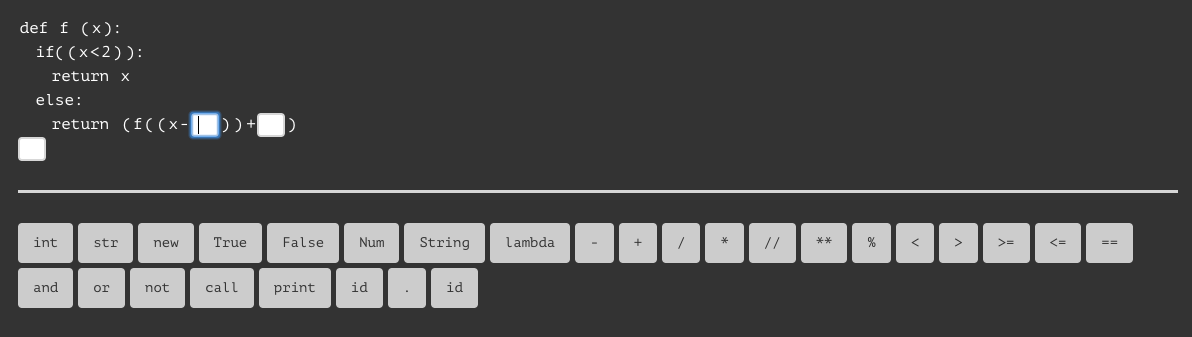
\includegraphics[width = 0.5\textwidth]{Figures/code_editor}
	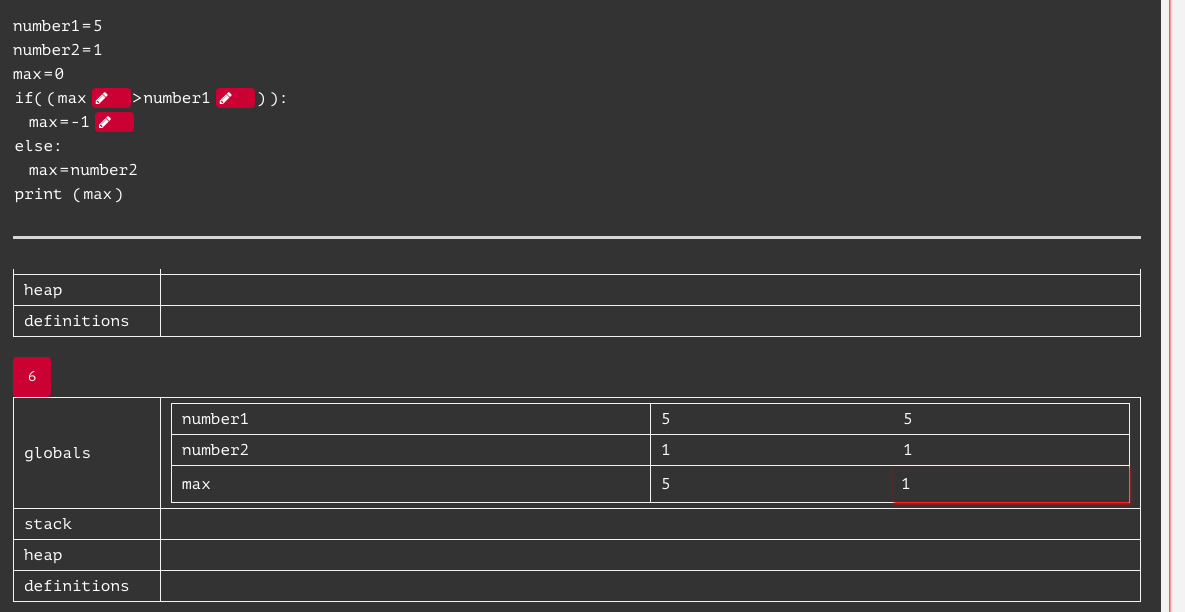
\includegraphics[width = 0.5\textwidth]{Figures/debugger}
	\caption{Code editor and debugger}
	\label{fig:code_editor_debugger}
\end{figure}

\begin{figure}
	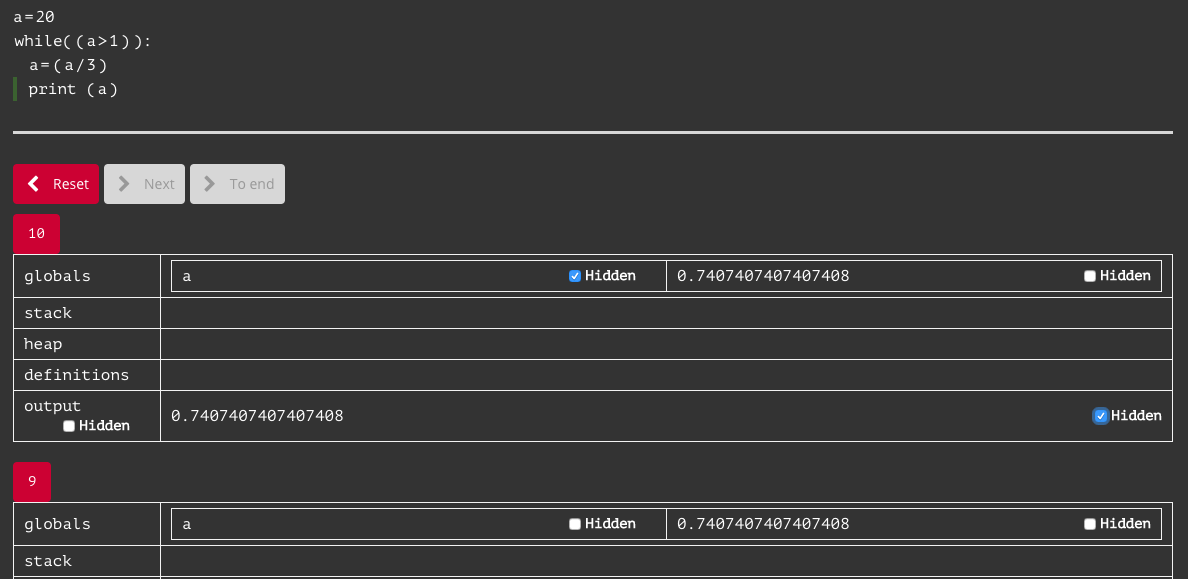
\includegraphics[width=0.5\textwidth]{Figures/forward_assignment}
	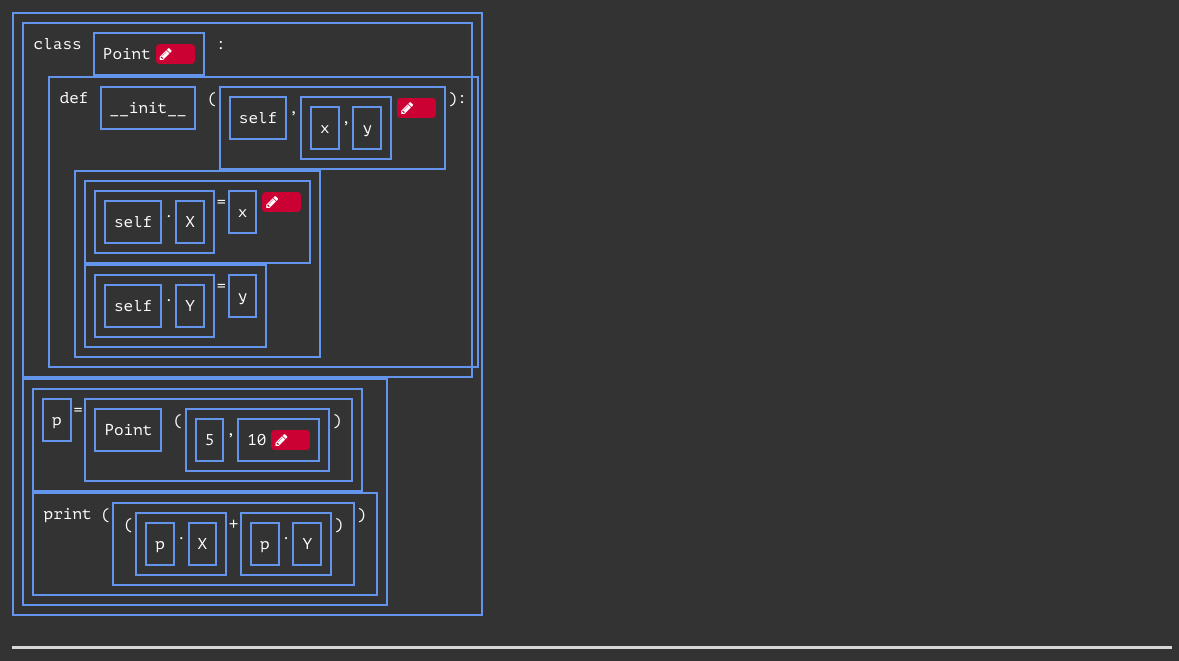
\includegraphics[width=0.5\textwidth]{Figures/backward_assignment}
	\caption{Teacher's assignment editor}
	\label{fig:assignment_editor}
\end{figure}

\begin{figure}
	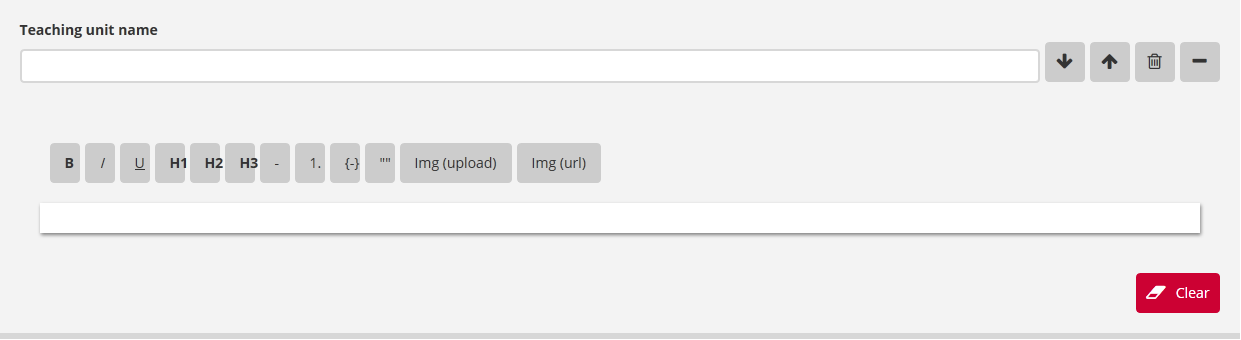
\includegraphics[width=0.5\textwidth]{Figures/slide_editor}
	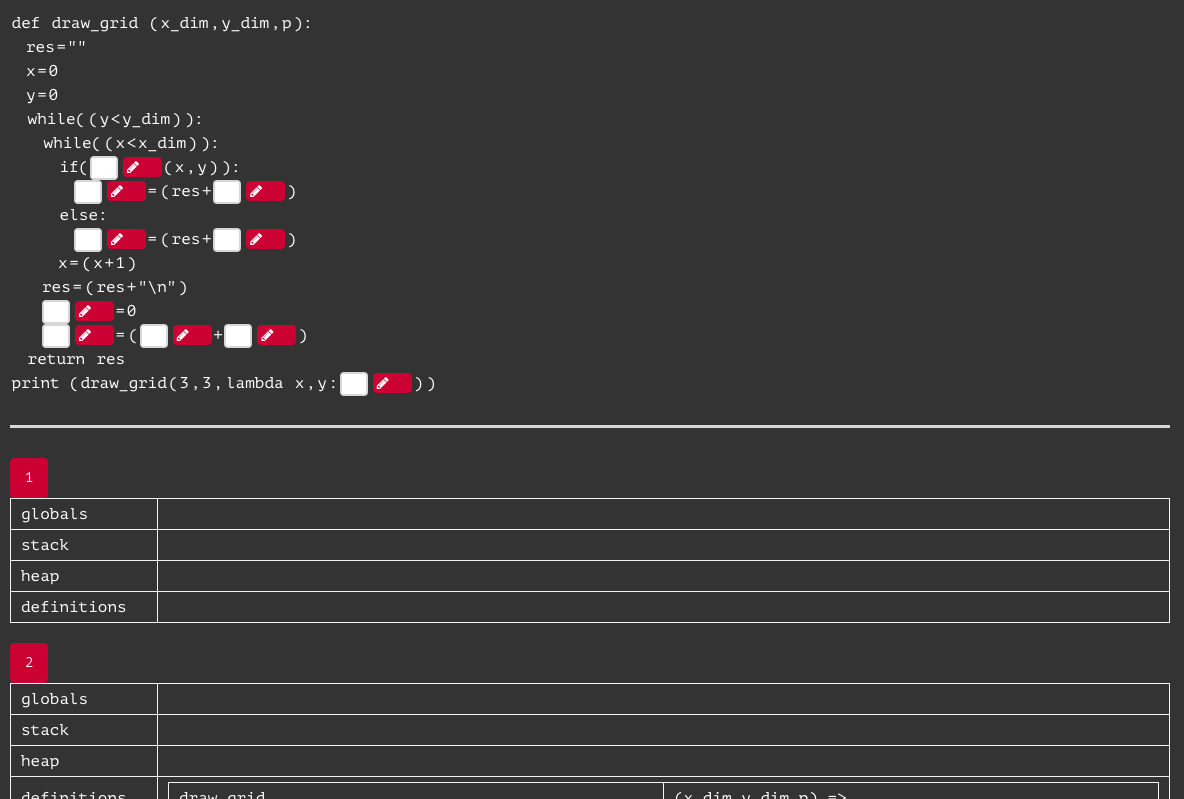
\includegraphics[width=0.5\textwidth]{Figures/forward_assignment_student}
	\caption{Slide editor and student's editor}
	\label{fig:slide_editor_student_editor}
\end{figure}

\subsection{Architecture}
In order to ensure the right level of responsivity, the application is features a large front-end written in React and TypeScript. React is a UI framework published by Facebook, implementing the functional reactive programming paradigm [...] in JavaScript and for browsers. The combination of referential transparency and controlled state updates make it possible to build truly complex, deeply hierarchical interactive structures with a high degree of correctness and confidence[add reference to referential transparency correctness]. TypeScript is an extension of JavaScript built by Microsoft, featuring a rich type-system inspired from the world of statically typed functional languages, emphasising inductive composition of types and generic programming. The combination of (functional) reactive programming and a rich language of statically checked types has enabled us to build a complex system with few defects and high performance and availability, without having to leave the platform of the web and therefore without sacrificing accessibility.

%insert schema of the architecture

The backend is twofold: on one hand we have a traditional Ruby on Rails application which is quite simple in its data storage and retrieval operations. On the other hand, the same code interpreter that powers the front-end is invoked by the backend in the form of a Nodejs service (Nodejs is a server-side JavaScript execution environment). By means of Nodejs, both the frontend and the backend feature the very same code interpreter, avoiding very unpleasant mismatches such as a correct answer on the front end which maps to a wrong answer according to the back end, and viceversa.

\subsection{The generic code interpreter}
The code interpreter is the beating heart of GrandeOmega. First of all, there is no “single programming language supported”: GrandeOmega is extensible to support any programming language definable: from Python (currently implemented), to SQL, and further to mathematical languages such as the lambda calculus or even languages for set theory and boolean logic.

The code interpreter is based on pattern matching and substitution and it directly mimic the small-step semantics [add reference] used to describe the formal semantics of computer languages. The small-step semantics define a set of rules in the form of logical rules, which means they are made of a (optional) set of premises that, if satisfied, will produce the result defined in the conclusion. If a rule does not contain premises it is called \textit{axiom} (meaning that its evaluation is immediate). Below you find an example of such rules describing the evaluation of the sum of two arithmetic expressions:

\begin{mathpar}
	\inferrule
	{ }
	{\langle \texttt{Integer x} \rangle \; \Rightarrow \; \texttt{Integer x}}
\end{mathpar}

\begin{mathpar}
	\inferrule
	{\langle \texttt{left} \rangle \; \Rightarrow \; \texttt{Integer x} \\\\
	 \langle \texttt{right} \rangle \; \Rightarrow \; \texttt{Integer y}}
	{\langle \texttt{left} + \texttt{right} \rangle \; \Rightarrow \; \texttt{Integer (x + y)}}
\end{mathpar}

The first rule is an axiom: if the input of the rule is an integer number \texttt{x} then its evaluation simply returns itself. The second rule evaluates the sum of two expressions by recursively calling the evaluation on the left and right expression. If the evaluation succeeds and returns an integer value, then the result of the whole rule is the arithmetic sum of the result of evaluating the two expressions.

From this example we proceed to define the general way of evaluating an semantics rule:

\begin{itemize}
	\item The left part of the conclusion is analysed by using pattern matching in the following way:
	\begin{itemize}
		\item If the current element is a variable then the pattern matching succeeds.
		\item If the current element is a constant we compare it with the input of the rule and if they are the same then the pattern matching succeeds.
		\item If the current element contains operators or other syntactical structures of the language (like the plus operator in the example), we compare the structure of the input of the rule with the one in the conclusion. This means that we check if the syntactical structure of the input of the rule is the same in the conclusion and then we check each argument of the syntactical structure by recursively applying these pattern matching steps.
	\end{itemize}
	\item We try to evaluate each one of the premises in the following way:
	\begin{itemize}
		\item We try to run each semantics rule in the language definition until one returns a result.
		\item If the result of a premise (right part of the arrow) is a specific syntactical structure then we test the pattern matching.
		\item If all the semantics rules fail to produce a suitable result then the current semantics rule fails to return a result.
	\end{itemize}
	\item We generate the result of the current semantics rule.
\end{itemize}

\subsection{The generic structured code editor}
Moreover, the code interpreter is not only involved in the evaluation of programs, but also in the rendering of their debugging steps, and in the interactive, structured editor.

[[Mudy: add explanation here and a couple of screenshots]]

